\chapter*{Studies}
\phantomsection

\addcontentsline{toc}{chapter}{Studies}

This chapter describes some side works, most of them incomplete, as a proposition or outline, but still in relation to or in the continuity of this writing.

\section*{Study 1 -- Entrelacs}
\phantomsection

\addcontentsline{toc}{section}{Study 1 -- Entrelacs}

This study consists of interlacing motivic patterns\footnote{See \texttt{interlace-cycle} in the Common Lisp library \textit{cl-cycle} and the method \texttt{interlace} in the SuperCollider extension \textbf{cycle}.} within a given \textit{ambitus}, according to other parameters such as the scale, the starting note, and the starting interval (toward upward scale if positive, or downward scale if negative), either as a musical score or as a process into the SuperCollider environment.

\subsection*{Generate Lilypond partition with Common Lisp}

Initially, this work was made in the PWGL\footnote{PWGL is a programming environment for an algorithmic composition written in the LISP programming language. It belongs to the Patch Work family initiated by Michael Laurson in 1985 including PatchWork and OpenMusic from the IRCAM and PWGL from the Sibelius Academy in Finland. Unfortunately, this software is not maintained anymore (the official website disappeared in 2020), but it is still possible to download it and to use it via emulation.} context as a package named \textit{Clavicorde}, just because the initial idea was to generate a score for clavicorde.

The idea then is to interlace two scales, one defined as the Messiaen mode 3 \texttt{(2 1 1 2 1 1 2 1 1)} and an original one \texttt{(5 6 3 10)}. Then, I choose to start each scale on the C note by octava (i.e. 4 octava as 4 voices recovered the clavicorde \textit{ambitus}), the two first ascending and the two last descending (by inverse intervals with \texttt{g-opposite}). 

\begin{figure}[htbp]
\begin{center}
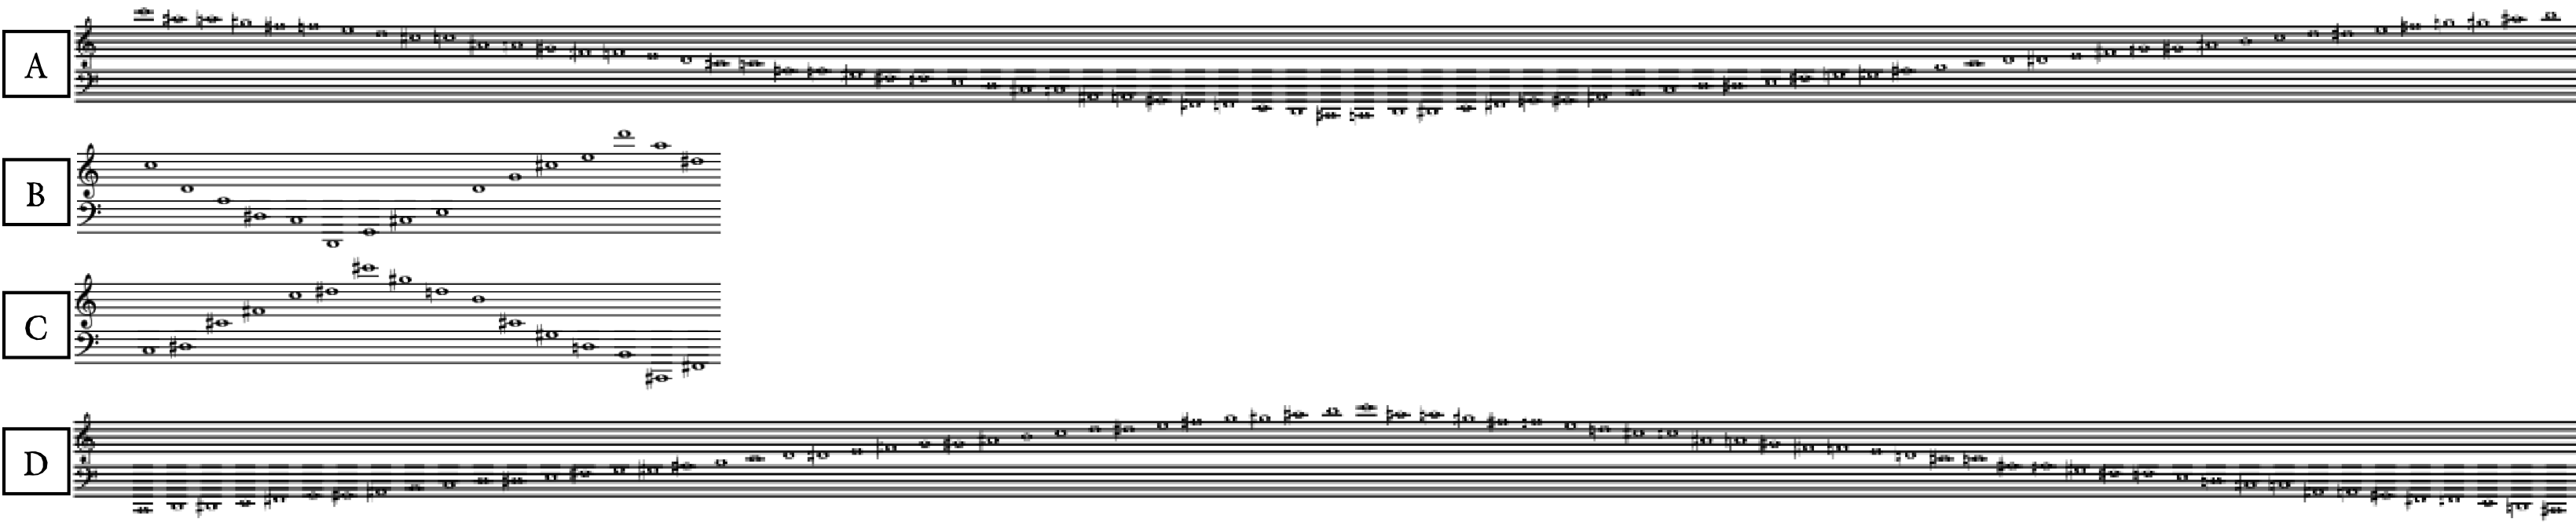
\includegraphics[width=\textwidth]{mp/img/scale}
\end{center}
\end{figure}

The Messiaen mode is wrapping the second scale. The latest need to be adjusted by a circular permutation (boxes \texttt{permut-circ}) to fit the cycle with the starting note (at least the closed one), then there are transposed (boxes \texttt{g+}) in order to start on the note C at the right octava. 

Note that the \textit{ambitus} (output of the \texttt{Chord-Editor}) is firstly set between C below F key (midi note 36) and C above G key (midi note 84). The real ambitus goes one tone beyond high C, that is to say, D (midi note 86), which is reached with the transposition of the two median scales.

\titlebox{\textit{\textbf{PWGL Clavicorde Patch}}}
{
\begin{center}
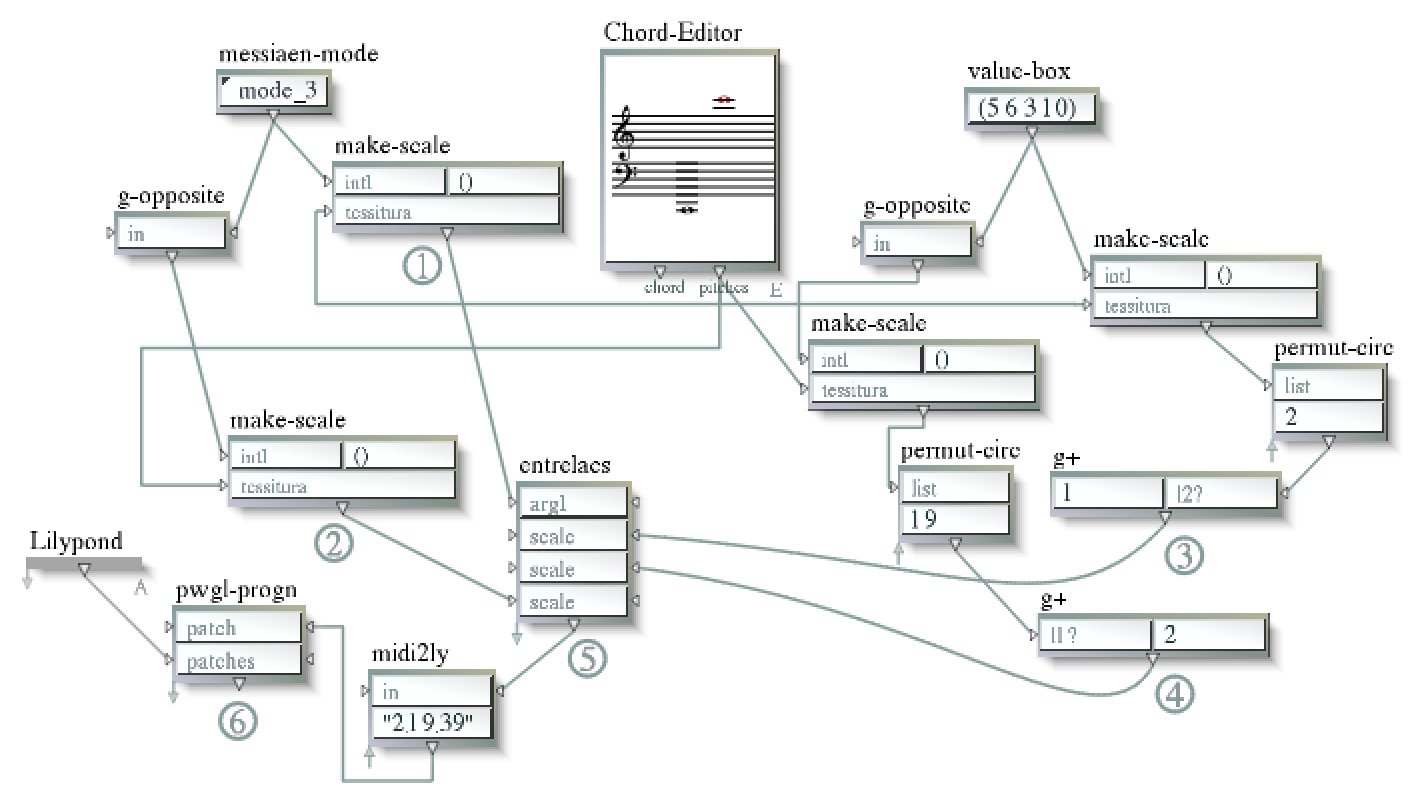
\includegraphics[width=\textwidth]{mp/img/patch}
\end{center}
} 

The previous scales are defined as \textcolor{gray}{\squared{A}}, \textcolor{gray}{\squared{B}}, \textcolor{gray}{\squared{C}}, and \textcolor{gray}{\squared{D}}, and the outputs of the boxes of the following patch, matches as follows:

\begin{description}
\item[ ] \textcolor{gray}{\circled{1}} $\rightarrow$ \textcolor{gray}{\squared{D}}
\item[ ] \textcolor{gray}{\circled{2}} $\rightarrow$ \textcolor{gray}{\squared{A}}
\item[ ] \textcolor{gray}{\circled{3}} $\rightarrow$ \textcolor{gray}{\squared{B}}
\item[ ] \textcolor{gray}{\circled{4}} $\rightarrow$ \textcolor{gray}{\squared{C}}
\end{description}

\smallskip

The output \textcolor{gray}{\circled{5}} applies the interlacing scales in such a way as to form a complete cycle by repeating 2 times \textcolor{gray}{\squared{A}} and \textcolor{gray}{\squared{D}}, and 9 times \textcolor{gray}{\squared{B}} and \textcolor{gray}{\squared{C}}.  

\bigskip

Then, \textcolor{gray}{\circled{6}} write the Lilypond file (generated with the function/box \texttt{midi2ly}) and export it as PDF (see PWGL Lilypond Abstraction box next page and the score in appendix page \pageref{clav}).

\titlebox{\textit{\textbf{PWGL Lilypond Abstraction}}}
{
\begin{center}
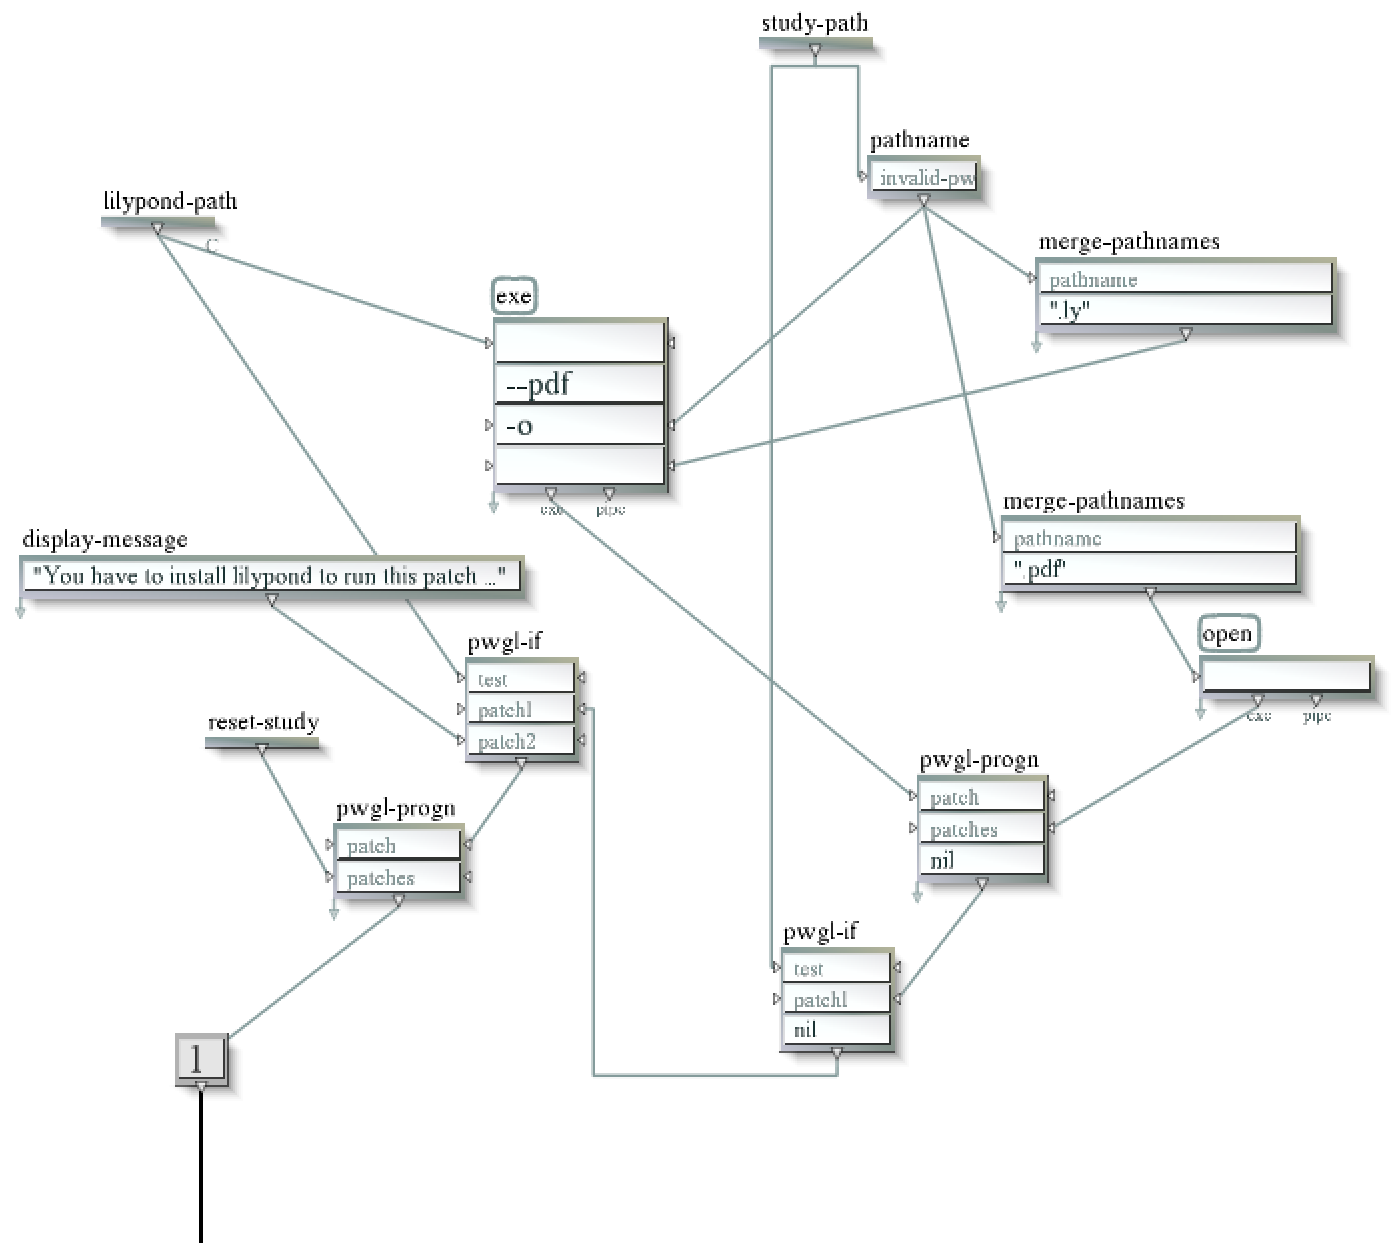
\includegraphics[width=\textwidth]{mp/img/lilypond-abs}
\end{center}
\vspace{-6mm}
} 

This was rather basic code and needed some \textit{ad hoc }adjustments. PWGL code has been therefore rewritten and improved in 'pure Common Lisp', completing some gap previously outlined, into the package \textit{cl-gsa} as the lisp file \textsf{studies.lisp}. The package \textit{cl-cycle}, as well as the generic package Lilypond, are required to generate the score for Clavicorde previously done in the PWGL context.

\bigskip
The function \texttt{make-scale} has been improved by adding two optional key parameters the midi root note (the minimal value of tessitura by default), and the beginning degree of the scale (0 by default).

\bigskip

As an example, and in order to explore the possibilities of this work, we reproduce the scales used in PWGL tutorial such as:

\begin{lstlisting}
(defvar *interlace*
  (cl-cycle:INTERLACE-CYCLE 
    (make-scale (messiaen-mode 3) :opp '(36 84))
    (make-scale '(5 6 3 10) :opp '(36 86) :root 37 :deg 2)
    (make-scale (opp '(5 6 3 10)) :opp '(36 86) :deg 3)
    (make-scale (opp (messiaen-mode 3)) :opp '(36 84))))
\end{lstlisting}
  
\begin{lstlisting}  
(entrelacs *interlace*
  :path "~/Desktop/entrelacs.ly"
  :title "Études"
  :subtitle "N°1 Entrelacs"
  :instrument "clavicorde"
  :composer "Yann Ics"
  :character "Vivacetto, leggiero e comodo"
  :endnote 
  "Cette étude représente un cycle formel. Les éventuelles 
   reprises sont laissé à la discrétion de l'interprète et 
   se font à partir de la barre de mesure en pointillé. 
   L'absence de la double barre de fin indique simplement
   le caractère cyclique de cette étude et suppose une 
   continuité hors de l'espace audible.")
\end{lstlisting}

\noindent The generated score is in the appendix page \pageref{clav}.

\bigskip

Obviously, this remains a work in progress, and some more keys need to be added to the function \texttt{entrelacs} to improve the score, like the key type according to the instrument, the open or the closed end bar (with or without coda), to name a few.

\subsection*{Generate SuperCollider process}

\begin{lstlisting}
~scale1 = [ 2, 1, 1, 2, 1, 1, 2, 1, 1 ];
~scale2 = [ 5, 6, 3, 10 ];

~entrelacs =
[
 [ 36, 84 ].cycleMidiScale(~scale1, ~scale1.reverse, 36),
 [ 36, 86 ].cycleMidiScale(~scale2, ~scale2.reverse, 37, 2),
 [ 86, 36 ].cycleMidiScale(~scale2.reverse, ~scale2, 38, 3),
 [ 84, 36 ].cycleMidiScale(~scale1.reverse, ~scale1, 36)
].interlace;

Pbind(\freq, Pseq(~entrelacs.flatten.midicps, inf), \dur, 0.2).play;
\end{lstlisting}

\bigskip

\section*{Study 2 -- Experimental Score Graph (ESG)}
\phantomsection

\addcontentsline{toc}{section}{Study 2 -- Experimental Score Graph (ESG)}

Convert an audio file to a graphical score with the analysis of \textsl{enkode}. The score reveals as such one aspect of the audio in terms of structure and/or form and can offer some interesting perspective as a concept for a musical interpretation.

\bigskip

\begin{lstlisting}
$ enkode -I '(5 3.5 3.5 4 4)' --loudness-diff-thres=1 
  --loudness-min-thres=2.5 --loudness-max-thres=15 
  --min-duration=0.1 --max-duration=5 --cutoff-frequency=100 
  --smooth-frequency=500 --time-step=0.01 
  .../audio.wav > data.enk
\end{lstlisting}

The arguments of \texttt{-I} refer respectively to a discrimination for:

\begin{itemize}
\item \textbf{duration} of 31 ($2^5 -1$) classes (because of the limited note values) as proportional notation, 
\item \textbf{f0} of 8 ($2^{\lfloor 3.5 \rfloor}$) classes (in order to fit inside the stave) as the number of different notes on the top stave,
\item \textbf{centroid} of 8 ($2^{\lfloor 3.5 \rfloor}$) classes (in order to fit inside the stave) as the number of different notes on the bottom stave,
\item \textbf{loudness} of 15 ($2^4 -1$) classes as the size of the note of the bottom stave,
\item \textbf{bass loudness} of 15 ($2^4 -1$) classes as the gray shade of the note of the bottom stave.
\end{itemize}
 
 \noindent
\begin{info}
\begin{minipage}{0.95\textwidth}
\vspace{0.2cm}
 So, the values of \texttt{-I} can't be modulated in order to fit the graphical constraints.
\vspace{0.2cm}
\end{minipage}
\end{info}

\begin{lstlisting}
;; generate lilypond file ...
CL-GSA> (score-graph ".../data.enk")
;; for details see comments in studies.lisp file
\end{lstlisting}

\noindent The generated score is in the appendix page \pageref{esg}.


%%%%%%%%%%%%%%%%%%%%%%%%%%%%%%%%
%%%%%%%%%%%%%%%%%%%%%%%%%%%%%%%%
%%%%%%%%%%%%%%%%%%%%%%%%%%%%%%%%
